\begin{center}
	
	\Huge
	Előerősítő 70\,cm-es sávra
	
	\Large
	\url{https://github.com/simonyiszk/70cm_preamp}
	
	\Large
	HA5KFU projekt
	
	\Large
	Kiss Ádám (HA8KDA), Bazsó Márton (HA7BM), \\ Keresztes Botond, Agócs Dániel, Pápay Levente (HA3PL)
\end{center}


\section*{Célkitűzés}

Az erősítő hivatása, hogy a Schönherz kollégium tetejére telepített 70\,cm-es sávra készült antenna által fogott jeleket erősítse, közülük is elsősorban a SMOG-1 műholdét 437,345\,MHz-en.


\section*{Kapcsolás}

Mivel az erősítő egy rádiófrekvencián elég "szennyezett" környékre kerül felszerelésre, így fontos egy jó szűrő alkalmazása ebben a fokozatban. Az akusztikus felületi hullámszűrők kitűnőek ilyen feladatokra, ugyanis nagyon meredek levágást biztosítanak a sávszéleken. Egy ilyen alkatrészt fellelni sem volt egyszerű, de beszerezni még bonyolultabbnak bizonyult, de végül a mouseren keresztül valahogyan sikerült. A választás az SF2446E\cite{SAW} néven futó áramkörre került, melynek a minimum beszerzési mennyisége 10\,db volt.

Mint a legtöbb vevőláncban itt is egy alacsony zajú előerősítő kerül a vételi lánc elejére. Előzőekben már épült egy hasonló kapcsolás egy ADL5523-as IC felhasználásával, de amikor kiderült, hogy az akusztikus szűrőből minimum 10-et kell rendelnünk, felmerült az ötlet, hogy gyártsunk le 10\,db áramkört, és a maradékra majd valahonnan kerítünk vevőt -- végül nem kellett sokat keresni, a nagy részük elkelt a klubon belül. Erősítőnek végül a Mini-Circuits PGA-103+\cite{PGA} terméke került kiválasztásra -- szintén a mouserről -- ugyanis kellően alacsony a zajtényezője, valamint 22\,dB erősítést ígér 400\,MHz-en, és végül, de nem utolsó sorban olcsóbb, mint egy ADL5523-as.

\begin{figure}[!ht]
	\centering
	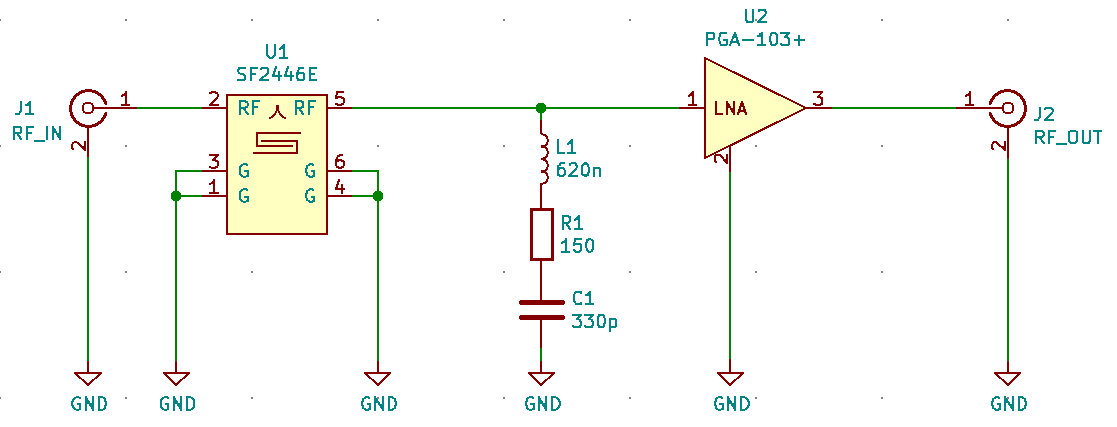
\includegraphics[keepaspectratio, width=0.8\textwidth]{kapcsolas.png}
	\caption{Az előerősítő kapcsolása}
	\label{fig:LNA_sch}
\end{figure}

Alapesetben az erősítő a szűrő elé kerülne, ugyanis az eredő rendszernek így kedvezőbb lesz a jel-zaj viszonya. Viszont mint említésre került, a telepítési hely RF szempontból elég "szennyezett", így félő, hogy a nagy sávszélességű erősítőnket könnyen túlvezérlik a számunkra érdektelen jelek. Ebből a meggondolásból a szűrőt az erősítő elé helyeztük, hogy csökkentsük a bele jutó összteljesítményt.

Amikor a NYÁK már majdnem gyártásba lett adva, Levente felhívta a figyelmünket egy kiegészítő dokumentumra\cite{PGA_comp}, mely az erősítőhöz megad egy kompenzáló hálózatot, ugyanis nélküle az áramkör 100\,MHz alatt nem lenne stabil. Így ez a 3 passzív alkatrészből álló kiegészítés az utolsó pillanatban még a tervre került. A végleges kapcsolás az \ref{fig:LNA_sch}-es ábrán látható.


\section*{NYÁK}

A hordozót elég kis méretűre meg lehetett csinálni, ugyanis mindösszesen 7 alkatrészt tartalmaz. A jelet vivő tápvonal úgy lett kialakítva, hogy a hullámimpedanciája 50\,$\Omega$-os legyen, ez főként azért lett ilyenre megcsinálva, hogy Marci gyakorolja CST-s szimulációs képességeit. Az elkészült rajzolat a \ref{fig:nyak}-es ábrán látható, mely egy kétrétegű, 1\,mm vastag hordozóra lett elkészítve.

\begin{figure}[!ht]
	\centering
	\begin{subfigure}[b]{0.49\textwidth}
		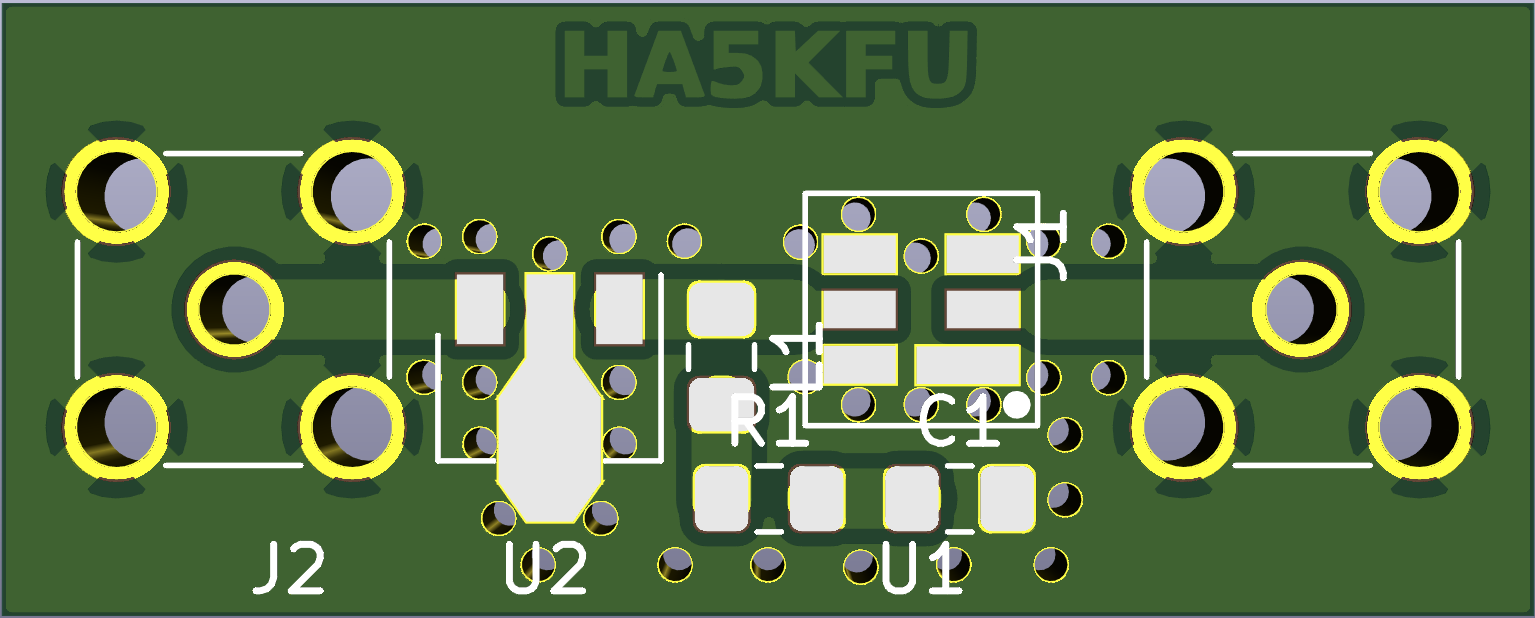
\includegraphics[keepaspectratio, width=\textwidth]{nyak_eleje.png}
		\caption{NYÁK eleje}
		\label{fig:nyak_elol}
	\end{subfigure}
	\begin{subfigure}[b]{0.49\textwidth}
		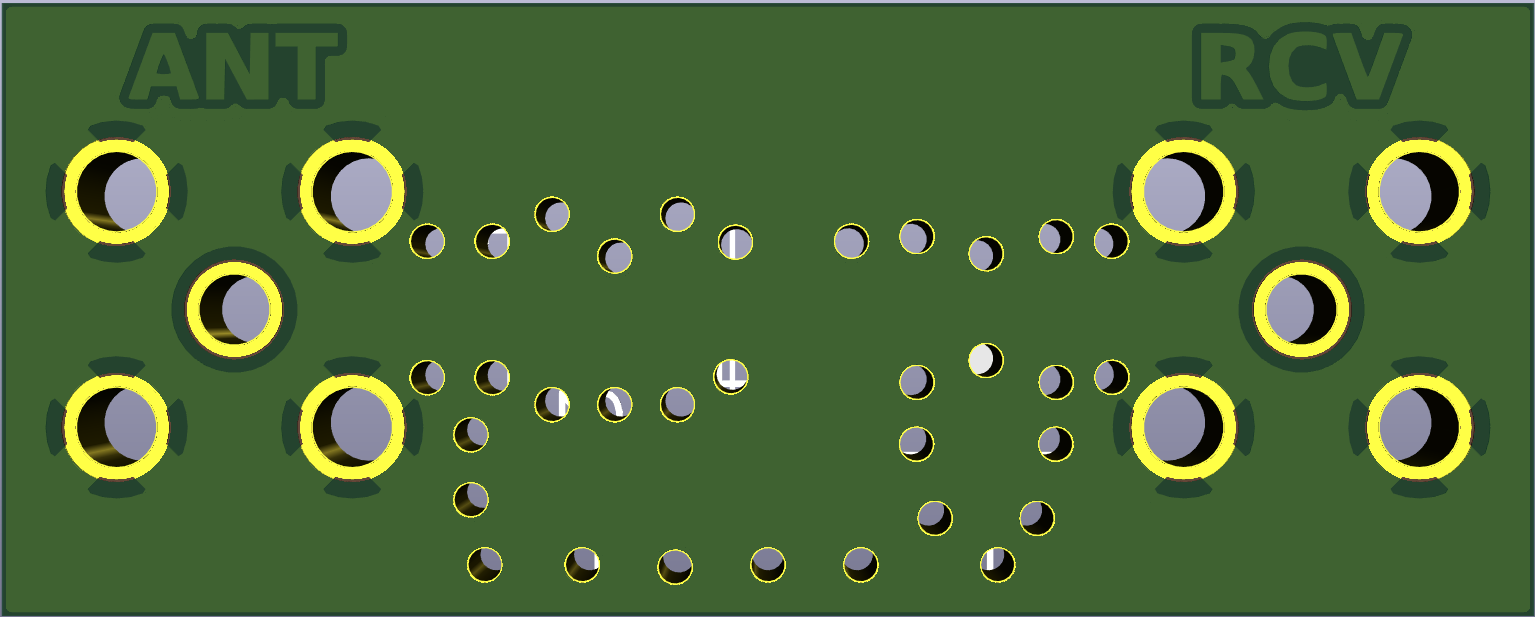
\includegraphics[keepaspectratio, width=\textwidth]{nyak_hatulja.png}
		\caption{NYÁK hátulja}
		\label{fig:nyak_hatul}
	\end{subfigure}
	\caption{NYÁK terv a KiCAD 3D nézetében}
	\label{fig:nyak}
\end{figure}

Némi megfontolást igényelt, hogy az áramkörünk hordozóját az Elektronikai Technológia Tanszéken, vagy egy keleti üzemben gyártassuk le. A döntő szempont végül a sebesség volt, ugyanis a SMOG-1 indítása rohamosan közeledett, és szerettünk volna elkészülni vele, így az ETT-re esett a választás, ugyanis a keletről történő postázás időtartama viszonylag hosszú és kiszámíthatatlan.


\section*{Mérések}

Miután elkészült néhány példány az áramkörből, ezek bemérésre kerültek a BME V1 épületében található Rohde \& Schwarz laboratóriumban egy vektor hálózat analizátoron, illetve mértünk rajtuk gerjedést az 1\,MHz - 1\,GHz tartományon egy jelanalizátorral, ezen mérési eredmények külön nem kerültek dokumentálásra. Az áramkörök táplálásához Yume tápfeladóját, és egy LM7805-öst használtunk.

A bemért áramkörök:

\begin{itemize}
	\item \#1 Szűrő + erősítő + kompenzáló hálózat
	\item \#2 Szűrő + erősítő + kompenzáló hálózat
	\item \#2.5 \#2-es áramkör javítás után (nem megfelelő forrasztás)
	\item \#3 Szűrő + erősítő
\end{itemize}

Mivel a klubban nem voltak fellelhetők a kompenzáló hálózathoz szükséges pontos értékek, így az a következő értékekkel lett megvalósítva:

\begin{itemize}
	\item L1 220\,nH
	\item R1 150\,$\Omega$
	\item C1 330\,pF
\end{itemize}

Az áramkörökről összesen 14 mérés készült (ebből 13-at le is mentettünk, az utolsót elfelejtettük). A következőkben a legfontosabbak kerülnek ismertetésre, a többit pedig a Függelék tartalmazza.

\subsection*{\#1-es áramkör}

A \ref{fig:erosito1}-as ábrán az áramkör átvitele ($S_{21}$ paraméter) látható.

\begin{figure}[!ht]
	\centering
	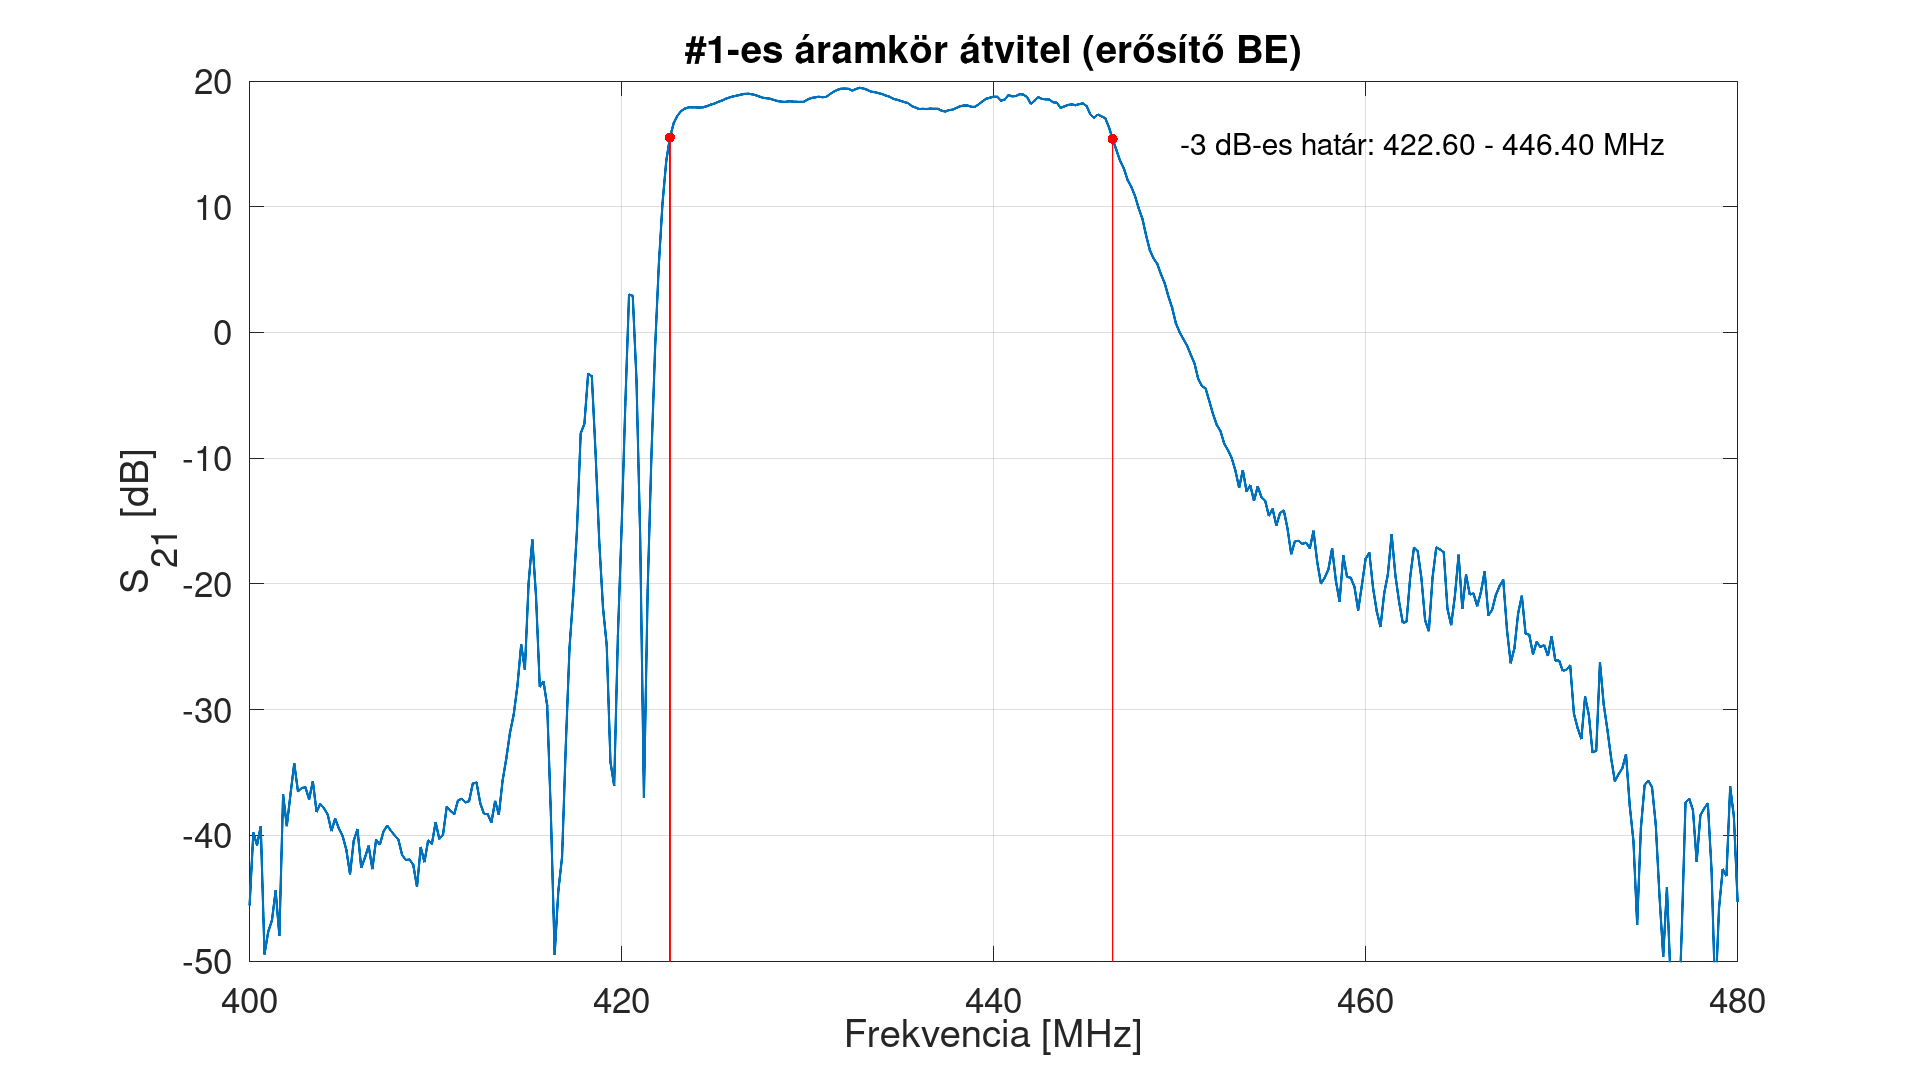
\includegraphics[keepaspectratio, width=\textwidth]{aramkor1_4.png}
	\caption{\#1-es erősítő átvitele}
	\label{fig:erosito1}
\end{figure}

A mérés nagyságrendileg megegyezik az elvárásokkal. Az erősítőtől ebben a tartományban 22\,dB erősítést várunk, míg a szűrő nagyjából 2\,dB-t csillapít, avagy közel a várt eredményt kaptuk. A sávszélesség is jól egyezik a szűrő adatlapjában\cite{SAW} megadott 23\,MHz-el, így összességében kijelenthető, hogy az áramkör az elvártnak megfelelően működik.

A vizsgálatok során nem találtunk gerjedésre utaló jeleket, így kijelenthető az is, hogy az alternatív értékekből összerakott kompenzáló hálózat is megfelelően ellátja feladatát.


\subsection*{\#2-es áramkör}

Ez az áramkör először nem működött rendeltetésszerűen, ugyanis az erősítése gyanúsan alacsony volt. Egy gyors mikroszkóp alatti szemrevételezés után kiderült, hogy ennek oka, a nem megfelelően beforrasztott erősítő volt. A hiba javítása után a \ref{fig:erosito2}-es ábrán látható átvitelt kaptuk.

\begin{figure}[!ht]
	\centering
	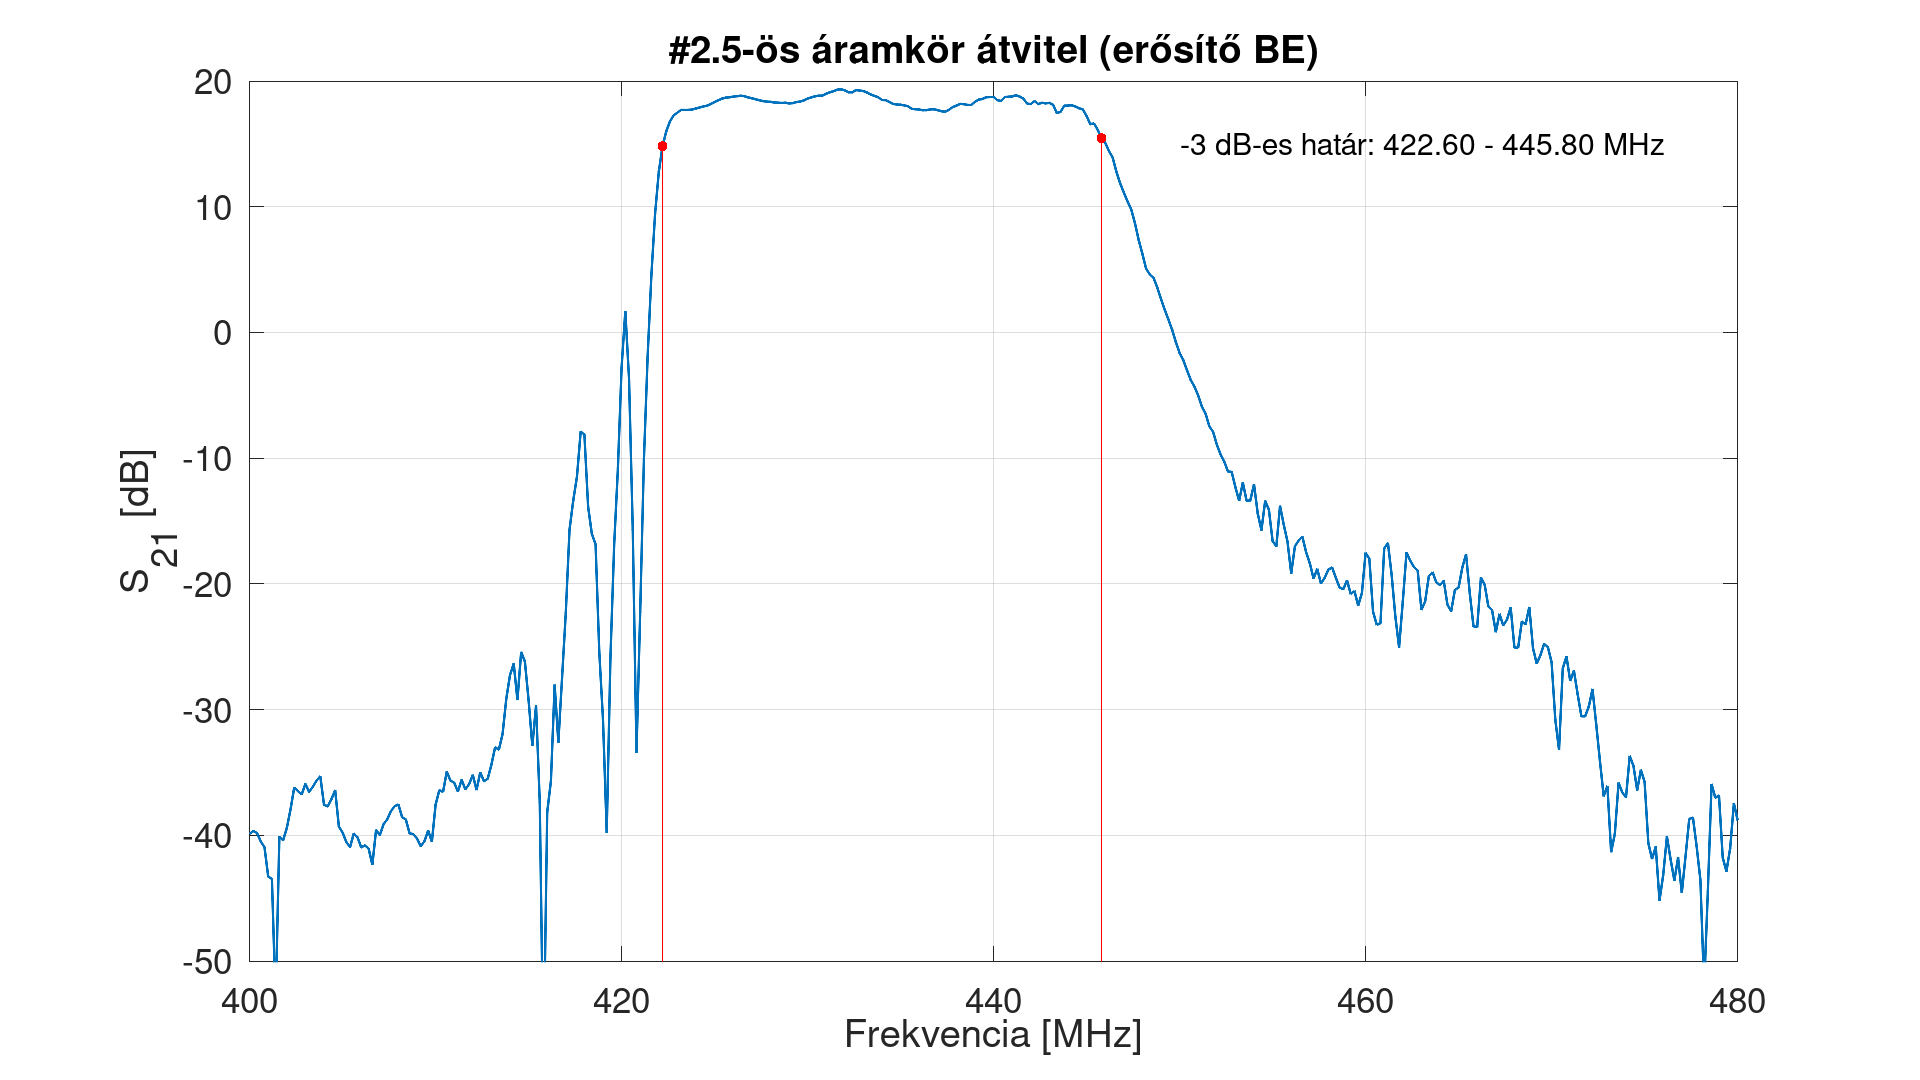
\includegraphics[keepaspectratio, width=\textwidth]{aramkor2_14.png}
	\caption{\#2.5-ös erősítő átvitele}
	\label{fig:erosito2}
\end{figure}

Látható, hogy az átvitel jellege megegyezik az \#1-es áramkörnél mérttel, így erről is elmondható, hogy megfelelően működik. Ez a kapcsolás eleinte mutatott gerjedés gyanús jeleket, melyeket a későbbiek során nem sikerült reprodukálnunk. Feltételezhetően a spektrumbeli kitüremkedések egy tranziensjelenség miatt következtek be. A további mérések során az áramkör stabilnak bizonyult.


\subsection*{\#3-as áramkör}

Miután megtaláltuk a kiegészítőt az adatlaphoz\cite{PGA_comp}, kíváncsiak voltunk, hogy vajon hogyan viselkedne az áramkör, ha nem építjük bele az ajánlott kompenzáló hálózatot. Ezért a harmadik áramkör csak a szűrő és az erősítőt tartalmazta. A mérés eredménye a \ref{fig:erosito3}-as ábrán látható.

\begin{figure}[!ht]
	\centering
	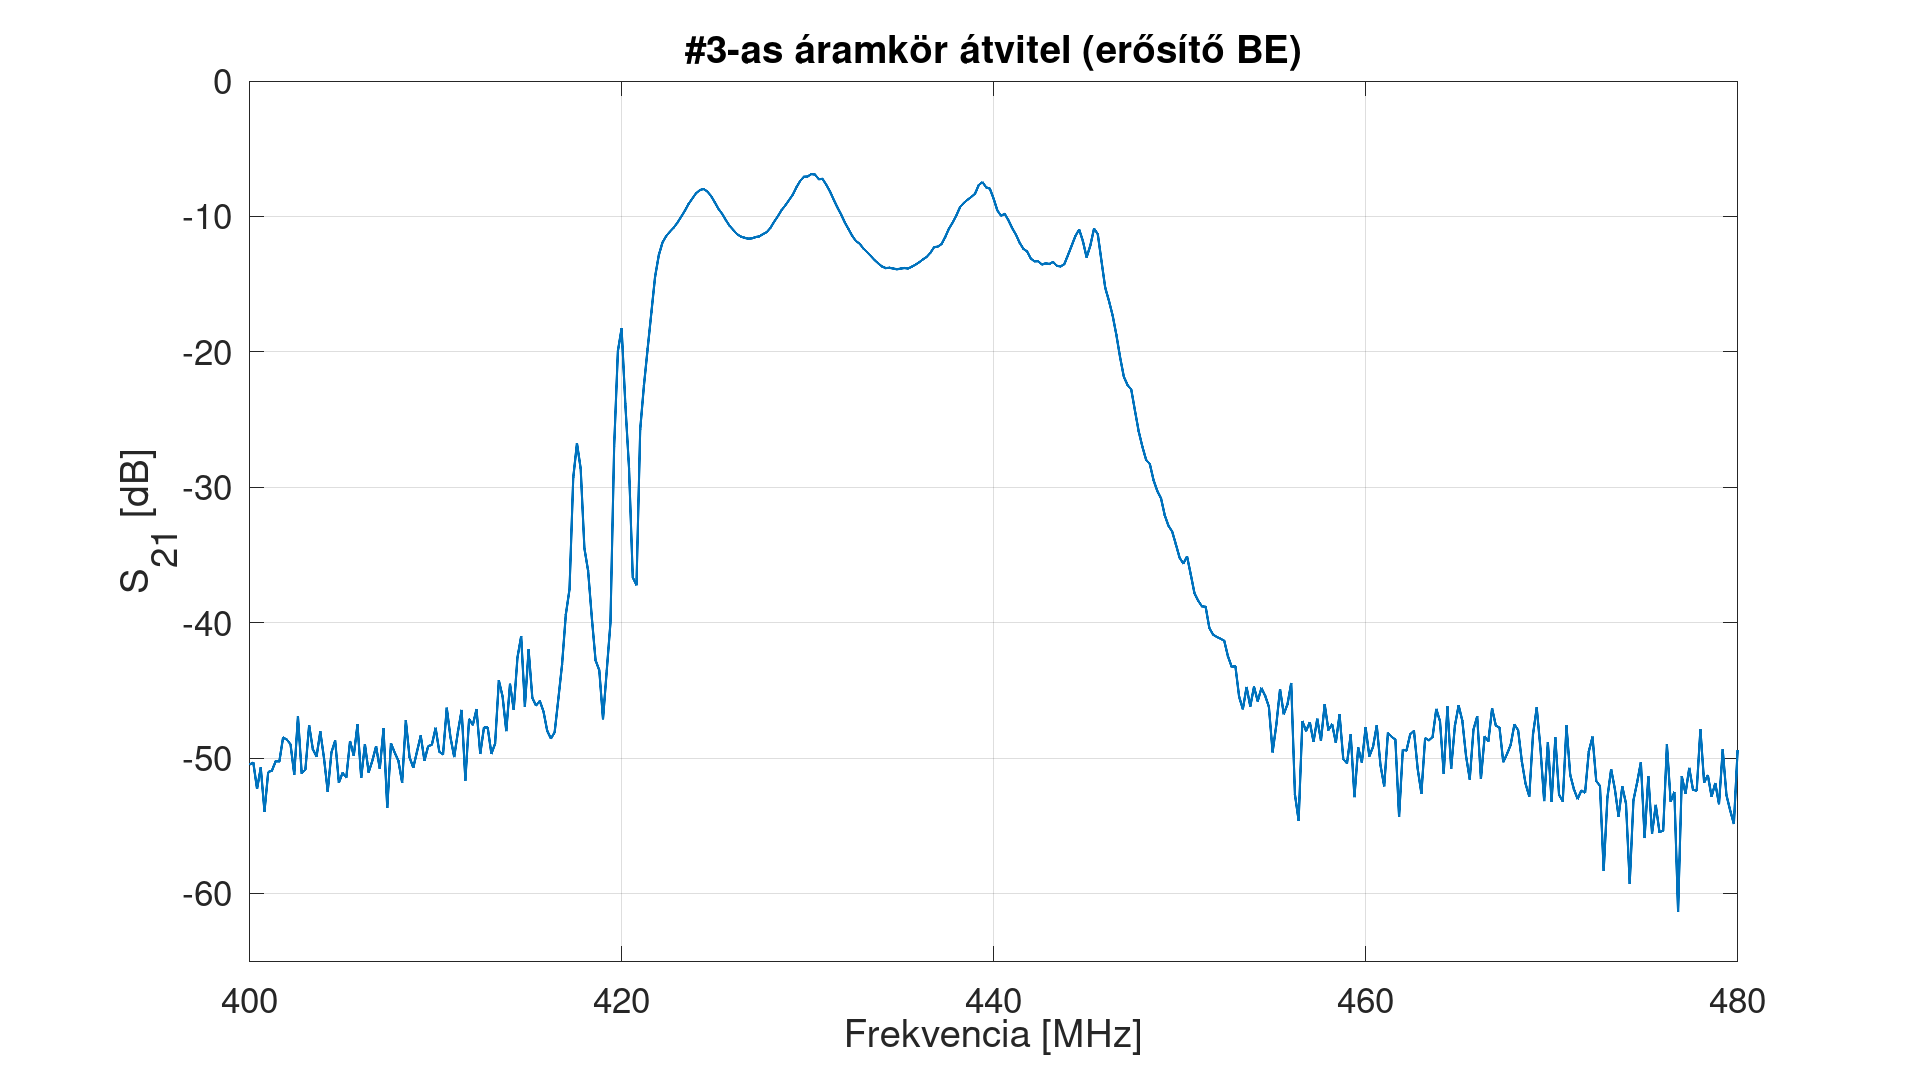
\includegraphics[keepaspectratio, width=\textwidth]{aramkor3_12.png}
	\caption{\#3-as erősítő átvitele}
	\label{fig:erosito3}
\end{figure}

Látszik, hogy a szűrő amplitúdómenete az áteresztő sávban jóval hullámosabb az adatlapban\,\cite{SAW} és az előző mérésekben látottnál. Ez a szűrő illesztetlenségére utalhat, ami azért különös, mert elméletileg minden eszközünk ki- és bemeneti impedanciája is 50\,$\Omega$-os. Látható az is, hogy az erősítő bekapcsolásakor is csak -10\,dB az átvitel, ami nem éppen nevezhető erősítőnek. Ezt a kapcsolást is megvizsgáltuk gerjedés szempontjából, de itt sem tapasztaltunk semmi ráutaló jelet.

1-2 nappal a mérések után felmerült bennem, hogy lehet, ennél a kapcsolásnál is volt nem megfelelő forrasztás, ugyanis szerintem a kompenzáló hálózat hiányának nem szabadna ekkora csillapítást okoznia (30\,dB-lel voltunk az elvárt szint alatt). A szűrőnek a megváltozott amplitúdómenetéből valószínűsíthető, hogy összességében a kompenzálóhálózat hiánya befolyással van az áramkör viselkedésére, viszont nem zárható ki, hogy volt egyéb tényező -- a kiegészítő hálózaton kívül -- ami befolyásolta az eredményt. Ezért szerintem nem jelenthető ki, hogy ez a mérés a kompenzáló hálózat átvitelre gyakorolt hatását szemlélteti.